\documentclass[a4paper]{article}

\usepackage[english]{babel}
\usepackage[utf8]{inputenc}
\usepackage{amsmath}
\usepackage{graphicx}
\usepackage{subfig}
\usepackage[colorinlistoftodos]{todonotes}
\setlength{\parindent}{0cm}
\setlength{\parskip}{3mm plus1mm minus1mm}

\title{Evolutionary approach for solving the Rubik’s Cube}

\author{Wojciech Krzystek, Jan Stypka}

\date{\today}

\begin{document}
\maketitle

\begin{abstract}
The Rubik's cube is both a very popular toy and an interesting mathematical problem. Many algorithms have already been developed to provide an efficient way of calculating the solution, one of them being the family of evolutionary strategies. Herdy's algorithm is a very interesting member of this family, because of its simplicity and good performance. In this paper we try to present this approach and propose a few different enhancements to this algorithm. We also provide test results in order to illustrate the influence of our enhancements.
\end{abstract}

\section{Introduction}
\subsection{Problem}

The Rubik’s cube has been a subject of scientific research for many years since its invention by Erno Rubik. It is a discrete combinatorial optimisation problem with a solution space of \(4.3*10^{19}\)different configurations, which makes it a non trivial game.

The point of the game is to arrange properly a coloured cube, so that each side (further on called face) is composed of small squares (facelets) in a single colour. The player is able to rotate each face either clockwise or counterclockwise in order to descramble the cube.
Usually the best solution is the one made quickest, but some variations of the game reward shortest solutions in favor of the complicated ones.

\subsection{Cube structure}
The classic \(3^3\) cube consists of  26 pieces: 8 corner pieces, 12 edge pieces and 6 center pieces. As previously mentioned, each side of a cube will be called face and each face is composed of 9 single-coloured facelets. The name cubie is introduced to denote a physical object, which can have 1 (middle cubie), 2 (edge cubie) or 3 (corner) visible facelets. The classic Rubik’s cube is composed of 26 such cubies.

Each face can be rotated clockwise (CW) or counterclockwise (CCW) thereby changing the position of its facelets. However, the facelet at the centre cannot be moved by any possible and legal rotation, thus determining the colour of a solved face.

In fact the middle row can be physically rotated, but such move is equivalent to rotating two surrounding faces in the opposite direction, hence the mutual location of the facelets in the centres is pre-determined.

For every corner and edge piece it is of great importance to distinguish between its position and orientation: i.e. an edge can be in a right position (defined by the two adjacent center colours), but in the wrong orientation.

\subsection{Notation}
There are 12 possible rotations at each point of the game - a clockwise and counterclockwise for each of the faces. To distinguish between them we will use a standard notation consisting of \textit{F, R, U, B, L, D}  which stand for front, right, up, back, left, down clockwise turn respectively and \textit{Fi, Ri, Ui, Bi, Li, Di} accordingly for the counterclockwise rotations. Therefore a single move can be described as one letter and a sequence by a string such as \textit{FBiDURi}.

We can also distinguish half-turns (\textit{F2, R2, U2, B2, L2, D2}), which are achieved by two consecutive quarter-turns, but are often perceived as a single move.

To complete this description, we should also mention the colours. Various implementations may differ, but we will use a fairly standard configuration: i.e. \textit{F = white, R = red, U = blue, B = yellow, L = orange, D = green}. 

\section{Original Herdy's algorithm}
\subsection{Individual representation}
An individual is represented by a list of rotations and a cube state. This state is equivalent to the initial problem tackled with the rotations from the list. To store the cube 6 two-dimensional (3x3) matrices are used.

\subsection{Mutation}
Although mutations that change the color of only a single facelet would be suitable for evolutionary algorithm, since they introduce steady change of fitness, they would yield non-existent cube states.

We could thread any valid single move, such as, for instance, Fi, as a mutation, but it would introduce too abrupt changes in fitness value.

It just so happens that it’s more effective in terms of evolutionary algorithm to thread sequences of multiple moves, well-known to cube solvers, which interchange the position of just few, say, 2 cubies, or rotate a single cubie.

Unfortunately these sequences comprise of multiple moves, yielding very long solutions from scrambled for solved cube. We sacrifice the length of final solution for the simplicity of the algorithm.

The sequences (mutations) are presented in the table \ref{table:mutations}

\begin{table}[h]
\caption{Possible mutations}
\label{table:mutations}
\begin{tabular}{l|l|c}
\textbf{Mutation} & \textbf{Sequence} & \textbf{Length} \\
\hline
two edge flip CW & FRBLULiUBiRiFiLiUiLUi & 14 \\
\hline
two edge flip CCW & FiLiBiRiUiRUiBLFRURiU & 14 \\
\hline
two corner flip CW & LDiLiFiDiFUFiDFLDLiUi & 14 \\
\hline
two corner flip CCW & RiDRFDFiUiFDiFiRiDiRU & 14 \\
\hline
three edge swap CW & UF2UiRiDiLiF2LDR & 10 \\
\hline
three edge swap CCW & UiF2ULDRF2RiDiLi & 10 \\
\hline
two edge/corner swap CW & RiURUiRiUFRBiRBRFiR2 & 14 \\
\hline
two edge/corner swap CCW & LUiLiULUiFiLiBLiBiLiFL2 & 14 \\
\hline
three corner swap CW & FiUBUiFUBiUi & 8 \\
\hline
three corner swap CCW & FUiBiUFiUiBU & 8 \\
\hline
three inslice edge swap CW & RLiU2RiLF2 & 6 \\
\hline
three inslice edge swap CCW & LiRU2LRiF2 & 6 \\
\end{tabular}
\end{table}

This table does not include “mirrors” of the listed sequences.
To take mirrors into account when performing a new mutation:
\begin{enumerate}
\item The face of the cube for which the sequence will be applied is chosen randomly (6 possibilities).
\item Next, the orientation of the cube is chosen (4 possibilities, each achieved by rotating the whole cube 0, 1, 2, or 3 quarter-turns clockwise).
\end{enumerate}
Altogether we have $ 12\cdot6\cdot4 = 288 $ possible mutations

\subsection{Fitness calculation}
Three qualities $ q1 $, $ q2 $, $ q3 $ are introduced:
\begin{itemize}
\item $ q1 $ is increased by 1 for each facelet whose color differs from the center facelet on the same face
\item $ q2 $ is increased by 4 for each wrong positioned edge, orientation is not considered
\item $ q3 $ is increased by 6 for each wrong positioned corner, orientation is not considered
\end{itemize}
Fitness is a sum of those 3 components. The lower the fitness = the better. Solved cube has fitness 0.

\subsection{Selection}
The original Herdy’s algorithm does not enforce any type of selection, but suggests that a simple elitist selection should yield best results. This type of selection consists of two steps:

\begin{enumerate}
\item Sorting the whole population by the fitness value
\item Choosing  best individuals (with the smallest fitness)
\end{enumerate}

This kind of selection guarantees preserving the best individuals, but has a negative impact on population diversity.

\section{Implemented enhancements}
We propose two enhancements to the described algorithm. The first is a little more complex tournament selection described in the subchapter below and the second one is an attempt to shrink developed solutions, which can be very long.

For all enhancements appropriate tests have been performed with the results presented in a separate chapter.

\subsection{Tournament selection}
This kind of selection is slightly more complex than a basic elitist selection. It consists of three basic steps:
\begin{enumerate}
\item Divide population into random several equally large groups
\item Choose the best individual in each group in terms of fitness value
\item Create a new population composed of these chosen individuals
\end{enumerate}

The strategy guarantees preserving the best individual for the whole population, but the other (second best, third best etc.) champions may not be chosen for the subsequent generation.
However, this method in certain circumstances enables the selection of worse individuals, which improves population diversity and may have a positive impact on the convergence speed.
This selection strategy also does not involve sorting and may perform better in terms of pure calculation speed.

\subsection{Solution reduction}
Second enhancement is an attempt to reduce the length of possible solutions. After each mutation an additional sequence of rotations is concatenated to the previous result yielding very long solutions after certain number of generations.

The only possibility of reducing the length of solution without introducing significant chances to the algorithm itself itself,
is to use the fact that 2 consecutive rotations in the opposite directions, performed on the same cube wall can be reduced to no rotation.

e.g. a sequence of rotations: 'LLBBiLiUiUR' can be reduced to: 'LR', however this is an extreme case: results indicate that this strategy reduces no more but by $5\%$.

\section{Tests}
\subsection{Parameters}
Basic parameters describing an evolutionary strategy are $(\mu, \lambda)$. The former defines the number of parents i.e. individuals selected from a population to give birth to another generation, while the latter parameter denotes offspring, that is the number of individuals generated from the previous population (parents).

Tests have been run to determine an optimal combination of $(\mu, \lambda)$ to carry out subsequent tests. Each value is an average of 10 different runs in order to gain statistical significance. The results are presented in the table \ref{table:params}.\todo{To fill!}

\begin{table}[h]
\centering
\caption{ $(\mu, \lambda)$ parameters}
\label{table:params}
\begin{tabular}{c|c|c|c}
& \textbf{100} & \textbf{200} & \textbf{500} \\
\hline
\textbf{10} & 12 & 12 & 12 \\
\hline
\textbf{20} & 14 & 14 & 14 \\
\hline
\textbf{50} & 15 & 15 & 15\\
\end{tabular}
\end{table}

The results indicate that pairs $(\mu, \lambda) = \{(x,y) : x \in \{1,2..3\} \wedge y \in \{5,6..7\}\}$ give the best performance, thus these values have been chosen for further testing.

Tests have been carried out to determine the behaviour of the algorithm, depending on the chosen selection and $(\mu, \lambda)$. The results are presented in tables \ref{table:elitist}, \ref{table:tournament}.


\subsection{Two possible approaches of measuring performance}
Since a lot of executions of the algorithm tend to settle in a local optimum (most often with fitness ranging from $10$ to $30$)
and not progress any further even after significant number of iterations, a limitation of iterations was introduced.
If the problem is not solved in this reasonable number of iterations, current evecution of the algorithm is aborted and reattempted.
2 approaches of masuring time performance are:
\begin{itemize}
	\item	take aborted runs into account: Since we need to make 10 successful runs, failed (stuck in a local optimum) runs are aborted,
			but time needed to perform this aborted run is added to the time of those 10 successful runs. It's ''fair'', since it matters if
			an algorithm can find a solution after 30 iterations, but more than a half of its runs end up as being aborted and the other algorithm
			is capable of finding a solution after 60 iterations, but only $10\%$ of its runs have to be terminated.
	\item   do not take aborted runs into account: Measure only the time needed to make 10 successfull runs.
\end{itemize}

\subsection{Elitist selection}

\begin{table}[h]
\centering
\caption{Elitist selection}
\label{table:elitist}
\subfloat[Average time]{
	\begin{tabular}{c|c|c|c}
	& \textbf{100} & \textbf{200} & \textbf{500} \\
	\hline
	\textbf{10} & 12 & 12 & 12 \\
	\hline
	\textbf{20} & 14 & 14 & 14 \\
	\hline
	\textbf{50} & 15 & 15 & 15\\
  \end{tabular}
}
\subfloat[Generations]{
	\begin{tabular}{c|c|c|c}
	& \textbf{100} & \textbf{200} & \textbf{500} \\
	\hline
	\textbf{10} & 12 & 12 & 12 \\
	\hline
	\textbf{20} & 14 & 14 & 14 \\
	\hline
	\textbf{50} & 15 & 15 & 15\\
  \end{tabular}
}
\end{table}


\subsection{Tournament selection}

\begin{table}[h]
\centering
\caption{Tournament selection}
\label{table:tournament}
\subfloat[Average time]{
	\begin{tabular}{c|c|c|c}
	& \textbf{100} & \textbf{200} & \textbf{500} \\
	\hline
	\textbf{10} & 12 & 12 & 12 \\
	\hline
	\textbf{20} & 14 & 14 & 14 \\
	\hline
	\textbf{50} & 15 & 15 & 15\\
  \end{tabular}
}
\subfloat[Generations]{
	\begin{tabular}{c|c|c|c}
	& \textbf{100} & \textbf{200} & \textbf{500} \\
	\hline
	\textbf{10} & 12 & 12 & 12 \\
	\hline
	\textbf{20} & 14 & 14 & 14 \\
	\hline
	\textbf{50} & 15 & 15 & 15\\
  \end{tabular}
}
\end{table}


\subsection{Solution reduction}

\todo{TODO}

\section{Conclusions}


----------------------

To na dole zostawiam, bo sie przydaje do przypominania komend latexowych



\section{Some \LaTeX{} Examples}
\label{sec:examples}

\subsection{How to Leave Comments}

Comments can be added to the margins of the document using the \todo{Here's a comment in the margin!} todo command, as shown in the example on the right. You can also add inline comments:

\todo[inline, color=green!40]{This is an inline comment.}

\subsection{How to Include Figures}

First you have to upload the image file (JPEG, PNG or PDF) from your computer to writeLaTeX using the upload link the project menu. Then use the includegraphics command to include it in your document. Use the figure environment and the caption command to add a number and a caption to your figure. See the code for Figure \ref{fig:frog} in this section for an example.

\begin{figure}
\centering
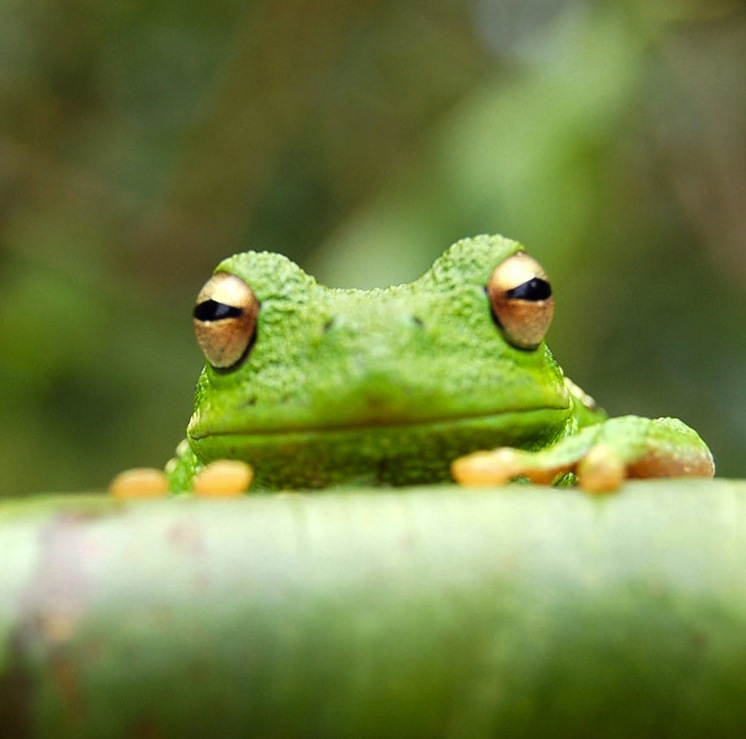
\includegraphics[width=0.3\textwidth]{frog.jpg}
\caption{\label{fig:frog}This frog was uploaded to writeLaTeX via the project menu.}
\end{figure}

\subsection{How to Make Tables}

Use the table and tabular commands for basic tables --- see Table~\ref{tab:widgets}, for example.

\begin{table}
\centering
\begin{tabular}{l|r}
Item & Quantity \\\hline
Widgets & 42 \\
Gadgets & 13
\end{tabular}
\caption{\label{tab:widgets}An example table.}
\end{table}

\subsection{How to Write Mathematics}

\LaTeX{} is great at typesetting mathematics. Let $X_1, X_2, \ldots, X_n$ be a sequence of independent and identically distributed random variables with $\text{E}[X_i] = \mu$ and $\text{Var}[X_i] = \sigma^2 < \infty$, and let
$$S_n = \frac{X_1 + X_2 + \cdots + X_n}{n}
      = \frac{1}{n}\sum_{i}^{n} X_i$$
denote their mean. Then as $n$ approaches infinity, the random variables $\sqrt{n}(S_n - \mu)$ converge in distribution to a normal $\mathcal{N}(0, \sigma^2)$.

\subsection{How to Make Sections and Subsections}

Use section and subsection commands to organize your document. \LaTeX{} handles all the formatting and numbering automatically. Use ref and label commands for cross-references.

\subsection{How to Make Lists}

You can make lists with automatic numbering \dots

\begin{enumerate}
\item Like this,
\item and like this.
\end{enumerate}
\dots or bullet points \dots
\begin{itemize}
\item Like this,
\item and like this.
\end{itemize}
\dots or with words and descriptions \dots
\begin{description}
\item[Word] Definition
\item[Concept] Explanation
\item[Idea] Text
\end{description}

We hope you find write\LaTeX\ useful, and please let us know if you have any feedback using the help menu above.

\end{document}